\documentclass[12pt, A4]{article}

% Packages
	% Basics
		\usepackage{amsmath}
		\usepackage{bm}
		\usepackage{cellspace}
		\usepackage{csquotes}
		\usepackage{fixltx2e}
		\usepackage[hang,flushmargin]{footmisc}
		\usepackage{float}
		\usepackage[margin=0.75in]{geometry}
		\usepackage{graphicx}
		\usepackage{hyperref}
		\usepackage[utf8]{inputenc}
		\usepackage{subcaption}
	% Diagrams
		\usepackage{pgfplots}
		\usepackage{tikz}
			\usepackage{circuitikz} % Circuits
			\usepackage{tikz-3dplot} % 3D
			\usetikzlibrary{arrows.meta, angles, calc, quotes}
	% Notation
		\usepackage{amssymb} % Miscellaneous
		\usepackage{chemformula}
		\usepackage{esint} % Integrals
		\usepackage{physics} % Differentials/Vectors
% Configuration
	\title{Differential Equations Project: Phase 4}
	\author{Arnav Patri and Shashank Chidige}
	\date{October 23, 2022}
	\hypersetup{
	    colorlinks,
	    citecolor=cyan,
	    filecolor=cyan,
	    linkcolor=cyan,
	    urlcolor=cyan
	}
	\cellspacetoplimit10pt
	\cellspacebottomlimit10pt
	
% Macros
	% Notation
		% Constants
			\DeclareMathOperator{\en}{e}
		% Distributions
			\newcommand{\Exp}{\mathbb{E}}
			\newcommand{\ndist}{\mathcal{N}}
			\DeclareMathOperator{\vari}{var}
		% Functions
			\DeclareMathOperator{\erfc}{erfc}
		% Sets
			\newcommand{\R}{\mathbb{R}}
		% Other
			\DeclareMathOperator{\avg}{avg}
			\renewcommand{\th}{\text{th}}
	% Utilities
		\newcommand{\callout}[2]{\begin{center}\fbox{\begin{minipage}{#1cm}#2\end{minipage}}\end{center}}
		\newcommand{\comment}[1]{}
		\newcommand{\subsectionb}[1]{\subsection*{#1}\addcontentsline{toc}{subsection}{#1}}
		\newcommand{\subsubsectionb}[1]{\subsubsection*{#1}\addcontentsline{toc}{subsubsection}{#1}}
		
\begin{document}
	\maketitle
	\noindent
		The following is the \href{https://docs.google.com/spreadsheets/d/10UhPew6GsC5f6DCJjFd24MZSaZ1SWjiQvmOD6k-tmcE/edit}{\underline{Excel spreadsheet}}. It uses data collected from Yahoo Finance on the value of GOOG (Alphabet Inc.'s stock price). \\
		A stock's price \(S_t\) (in USD) can be predicted with respect to time \(t\) (in days from an initial time) using a growth function; that is, by relating the rate at which the stock price is changing to the current stock price as a proportion:
			\[\dv{S_t}{t} \propto S_t\]
			The constant of proportionality is the drift \(\mu\) of the stock, which is the rate of change of the expected value \(\Exp[S_t]\) of the stock price with respect to time (which is not the expected value of its rate of change):
			\[
				\dv{S_t}{t} = \mu S_t \qquad \text{where} \qquad
				\mu= \frac{\Delta \Exp[S_t]}{\Delta t}
			\]
			The stock market is constantly volatile, though, changing in unpredictable ways. This randomness element can be modeled by a randomness term, proportional to the product of the stock price and the rate of change of the standard Wiener process \(W_t\) (as defined in Phase 2):
			\[\text{rate of randomness} \propto S_t\dv{W_t}{t}\]
			The proportionality constant is the volatility \(\sigma\) of the stock, which is simply its standard deviation. Adding this term,
			\[
				\dv{S_t}{t} = \mu S_t + \sigma S_t\dv{W_t}{t} \qquad \text{where} \qquad
				\sigma = \frac{\sum (S_{t, i} - \bar{S_t})}{n - 1} \qquad \text{and} \qquad
				\bar{S_t} = \frac{\sum S_{t, i}}{n}
			\]
			The randomness term ensures that each trial of the model yields a different graph. One such trial is attached at the end of this document.
		The DE can be rewritten as
			\[\dd{S}_t = \mu_t\dd{t} + \sigma_t\dd{W_t}\]
			where \(\mu_t = \mu S_t\) and \(\sigma_t = \sigma S_t\). Integrating and reparameterizing \(\mu_t\), \(\sigma_t\) and \(W_t\) with \(s\),
			\[S_t = \int_0^t\mu_s\dd{s} + \int_0^t\sigma_s\dd{W}_s + S_0\]
			where \(S_0\) is the constant of integration (the initial stock price). This makes \(S_t\) an It\^o process, a stochastic process expressible as the sum of two integrals, one with respect to a stochastic process and another with respect to time, and a constant. \\
		The Taylor expansion of a twice-differentiable scalar function \(f(t, s)\) is
			\[\dd{f} = \pdv{f}{t}\dd{t} + \pdv{f}{s}\dd{s} + \frac{1}{2}\pdv[2]{f}{s}\dd[2]{s} + \cdots\]
			Substituting \(S_t\) for \(s\) and appropriately substituting for \(\dd{s}\) yields
			\[\dd{f} + \pdv{f}{t}\dd{t} + \pdv{f}{s} (\mu_t\dd{t} + \sigma_t\dd{W_t}) + \pdv[2]{f}{s}\left(\mu_t^2\dd{t^2} + 2\mu_t\sigma_t\dd{t}\dd{W_t} + \sigma_t^2\dd{W_t}^2\right) + \cdots\]
			As \(\dd{t}\) approaches 0, \(\dd{t}^2\) and \(\dd{t}\dd{W_t}\) tend to zero faster than \(\dd{W_t^2}\). Substituting 0 for \(\dd{t^2}\) and \(\dd{t}\dd{W_t}\) and \(\dd{t}\) for \(\dd{W_t^2}\) yields
			\[\dd{f} = \left(\pdv{f}{t} + \mu_t\pdv{f}{s} + \frac{\sigma_t^2}{2}\pdv[2]{f}{s}\right)\dd{t} + \sigma_t\pdv{f}{s}\dd{W_t}\]
			This is itself an It\^o process. It\^o's lemma states that for any It\^o process \(S_t\) and any twice-differentiable function \(f(t, s)\), \(f(t, S_t)\) is an It\^o process. \\
		Let \(f(S_t) = \ln S_t\). Applying It\^o's lemma,
			\begin{align*}
				\dd{f} &= f'(S_t)\dd{S_t} + \frac{1}{2}f''(S_t)(\dd{S_t})^2 \\
					&= \frac{1}{S_t}\dd{S_t} - \frac{1}{2S_2^2}\left(S_t^2\sigma^2\dd{t}\right) \\
					&= \frac{1}{S_t}(\sigma S_1 \dd{W_t} + \mu S_t \dd{t}) - \frac{\sigma^2}{2}\dd{t} \\
					&= \sigma \dd{W_t} + \left(\mu - \frac{\sigma^2}{2}\right)\dd{t}
			\end{align*}
			Integrating the separable DE,
			\[
				f(t) = \ln S_t 
					= \ln S_0 + \sigma W_t + \left(\mu - \frac{\sigma^2}{2}\right)\dd{t} \\
			\]
			This can finally be exponentiated, yielding \(S_t\):
			\[S_t = S_0\en^{\left(\mu - \frac{\sigma^2}{2}\right)t + \sigma W_t}\]
			(This solution was largely adapted from \href{https://pi.math.cornell.edu/~web6720/Wendy_slides.pdf}{\underline{Introduction to Ito's Lemma}} by Wenyu Zhang and \\\href{https://medium.com/the-quant-journey/a-gentle-introduction-to-geometric-brownian-motion-in-finance-68c37ba6f828}{\underline{A Gentle Introduction to Geometric Brownian Motion in Finance}} by Andrea Chello.) \\
			Substituting for \(S_0\), \(\mu\), and \(\sigma\) (using the values derived in Phase 3),
			\[S_t = 141.501\en^{\left(0.00064 + \frac{4.356^2}{2}\right)t + 4.356W_t} = 141.501\en^{9.488t + 4.356W_t}\]
			The only condition this model must meet is the initial stock price being \$141.501, which is satisfied by setting the integration constant \(S_0\) to it. It should also be noted that the Stock's price may not fall below 0, as the solution is an exponential with a positive coefficient. \\
			The following are the MatLab code, solution (for the deterministic term), and graph of the model of \(S_t\) vs \(t\):
				\[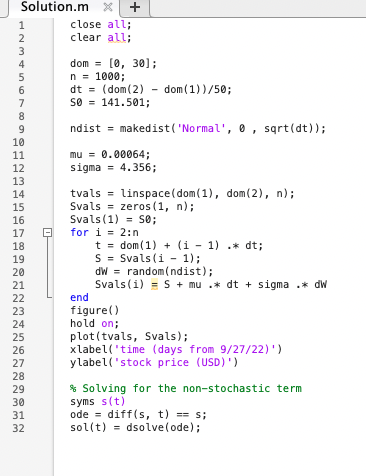
\includegraphics[width = 8cm]{Images/matlab.png}\]
				\[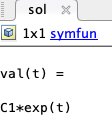
\includegraphics[width = 2cm]{Images/sol.png}\]
				\[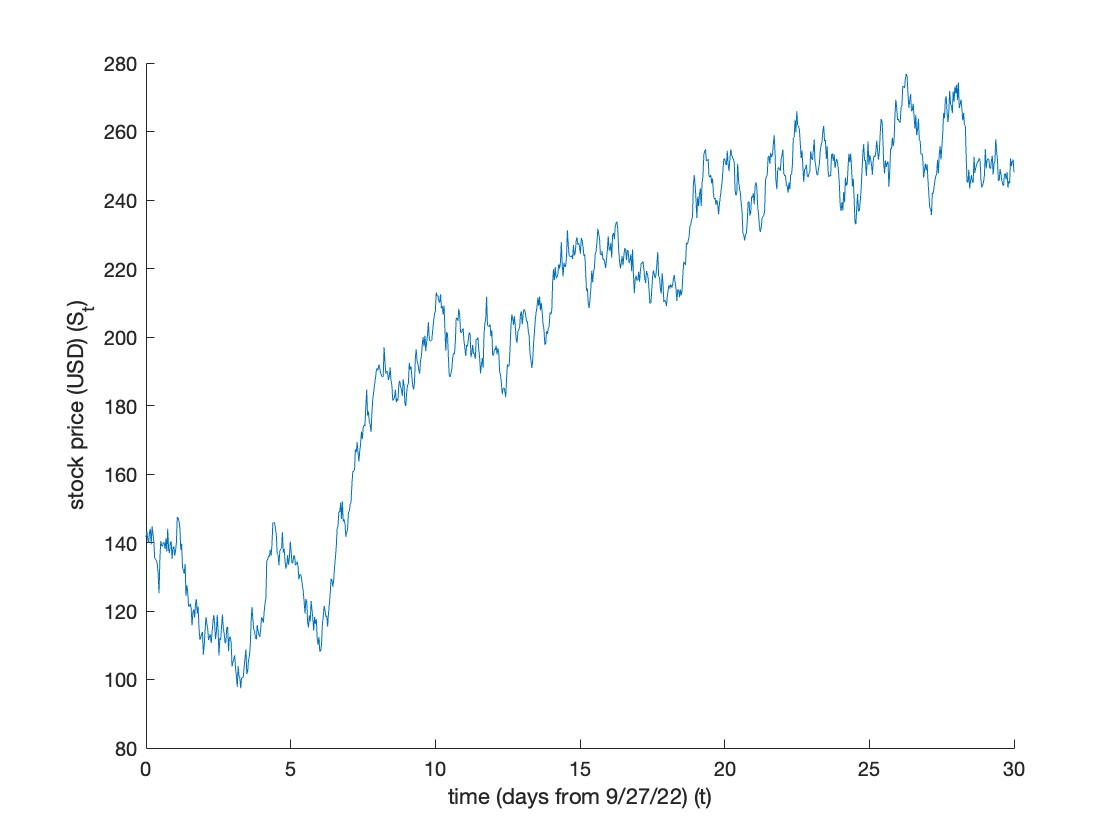
\includegraphics[width = 10cm]{Images/modelGraph.jpg}\]
			
\end{document}